\documentclass[]{article}
\usepackage{lmodern}
\usepackage{amssymb,amsmath}
\usepackage{ifxetex,ifluatex}
\usepackage{fixltx2e} % provides \textsubscript
\ifnum 0\ifxetex 1\fi\ifluatex 1\fi=0 % if pdftex
  \usepackage[T1]{fontenc}
  \usepackage[utf8]{inputenc}
\else % if luatex or xelatex
  \ifxetex
    \usepackage{mathspec}
  \else
    \usepackage{fontspec}
  \fi
  \defaultfontfeatures{Ligatures=TeX,Scale=MatchLowercase}
\fi
% use upquote if available, for straight quotes in verbatim environments
\IfFileExists{upquote.sty}{\usepackage{upquote}}{}
% use microtype if available
\IfFileExists{microtype.sty}{%
\usepackage{microtype}
\UseMicrotypeSet[protrusion]{basicmath} % disable protrusion for tt fonts
}{}
\usepackage[margin=1in]{geometry}
\usepackage{hyperref}
\hypersetup{unicode=true,
            pdftitle={Spicy Burger Roulette},
            pdfauthor={Sean Soutar},
            pdfborder={0 0 0},
            breaklinks=true}
\urlstyle{same}  % don't use monospace font for urls
\usepackage{color}
\usepackage{fancyvrb}
\newcommand{\VerbBar}{|}
\newcommand{\VERB}{\Verb[commandchars=\\\{\}]}
\DefineVerbatimEnvironment{Highlighting}{Verbatim}{commandchars=\\\{\}}
% Add ',fontsize=\small' for more characters per line
\usepackage{framed}
\definecolor{shadecolor}{RGB}{248,248,248}
\newenvironment{Shaded}{\begin{snugshade}}{\end{snugshade}}
\newcommand{\KeywordTok}[1]{\textcolor[rgb]{0.13,0.29,0.53}{\textbf{#1}}}
\newcommand{\DataTypeTok}[1]{\textcolor[rgb]{0.13,0.29,0.53}{#1}}
\newcommand{\DecValTok}[1]{\textcolor[rgb]{0.00,0.00,0.81}{#1}}
\newcommand{\BaseNTok}[1]{\textcolor[rgb]{0.00,0.00,0.81}{#1}}
\newcommand{\FloatTok}[1]{\textcolor[rgb]{0.00,0.00,0.81}{#1}}
\newcommand{\ConstantTok}[1]{\textcolor[rgb]{0.00,0.00,0.00}{#1}}
\newcommand{\CharTok}[1]{\textcolor[rgb]{0.31,0.60,0.02}{#1}}
\newcommand{\SpecialCharTok}[1]{\textcolor[rgb]{0.00,0.00,0.00}{#1}}
\newcommand{\StringTok}[1]{\textcolor[rgb]{0.31,0.60,0.02}{#1}}
\newcommand{\VerbatimStringTok}[1]{\textcolor[rgb]{0.31,0.60,0.02}{#1}}
\newcommand{\SpecialStringTok}[1]{\textcolor[rgb]{0.31,0.60,0.02}{#1}}
\newcommand{\ImportTok}[1]{#1}
\newcommand{\CommentTok}[1]{\textcolor[rgb]{0.56,0.35,0.01}{\textit{#1}}}
\newcommand{\DocumentationTok}[1]{\textcolor[rgb]{0.56,0.35,0.01}{\textbf{\textit{#1}}}}
\newcommand{\AnnotationTok}[1]{\textcolor[rgb]{0.56,0.35,0.01}{\textbf{\textit{#1}}}}
\newcommand{\CommentVarTok}[1]{\textcolor[rgb]{0.56,0.35,0.01}{\textbf{\textit{#1}}}}
\newcommand{\OtherTok}[1]{\textcolor[rgb]{0.56,0.35,0.01}{#1}}
\newcommand{\FunctionTok}[1]{\textcolor[rgb]{0.00,0.00,0.00}{#1}}
\newcommand{\VariableTok}[1]{\textcolor[rgb]{0.00,0.00,0.00}{#1}}
\newcommand{\ControlFlowTok}[1]{\textcolor[rgb]{0.13,0.29,0.53}{\textbf{#1}}}
\newcommand{\OperatorTok}[1]{\textcolor[rgb]{0.81,0.36,0.00}{\textbf{#1}}}
\newcommand{\BuiltInTok}[1]{#1}
\newcommand{\ExtensionTok}[1]{#1}
\newcommand{\PreprocessorTok}[1]{\textcolor[rgb]{0.56,0.35,0.01}{\textit{#1}}}
\newcommand{\AttributeTok}[1]{\textcolor[rgb]{0.77,0.63,0.00}{#1}}
\newcommand{\RegionMarkerTok}[1]{#1}
\newcommand{\InformationTok}[1]{\textcolor[rgb]{0.56,0.35,0.01}{\textbf{\textit{#1}}}}
\newcommand{\WarningTok}[1]{\textcolor[rgb]{0.56,0.35,0.01}{\textbf{\textit{#1}}}}
\newcommand{\AlertTok}[1]{\textcolor[rgb]{0.94,0.16,0.16}{#1}}
\newcommand{\ErrorTok}[1]{\textcolor[rgb]{0.64,0.00,0.00}{\textbf{#1}}}
\newcommand{\NormalTok}[1]{#1}
\usepackage{graphicx,grffile}
\makeatletter
\def\maxwidth{\ifdim\Gin@nat@width>\linewidth\linewidth\else\Gin@nat@width\fi}
\def\maxheight{\ifdim\Gin@nat@height>\textheight\textheight\else\Gin@nat@height\fi}
\makeatother
% Scale images if necessary, so that they will not overflow the page
% margins by default, and it is still possible to overwrite the defaults
% using explicit options in \includegraphics[width, height, ...]{}
\setkeys{Gin}{width=\maxwidth,height=\maxheight,keepaspectratio}
\IfFileExists{parskip.sty}{%
\usepackage{parskip}
}{% else
\setlength{\parindent}{0pt}
\setlength{\parskip}{6pt plus 2pt minus 1pt}
}
\setlength{\emergencystretch}{3em}  % prevent overfull lines
\providecommand{\tightlist}{%
  \setlength{\itemsep}{0pt}\setlength{\parskip}{0pt}}
\setcounter{secnumdepth}{0}
% Redefines (sub)paragraphs to behave more like sections
\ifx\paragraph\undefined\else
\let\oldparagraph\paragraph
\renewcommand{\paragraph}[1]{\oldparagraph{#1}\mbox{}}
\fi
\ifx\subparagraph\undefined\else
\let\oldsubparagraph\subparagraph
\renewcommand{\subparagraph}[1]{\oldsubparagraph{#1}\mbox{}}
\fi

%%% Use protect on footnotes to avoid problems with footnotes in titles
\let\rmarkdownfootnote\footnote%
\def\footnote{\protect\rmarkdownfootnote}

%%% Change title format to be more compact
\usepackage{titling}

% Create subtitle command for use in maketitle
\newcommand{\subtitle}[1]{
  \posttitle{
    \begin{center}\large#1\end{center}
    }
}

\setlength{\droptitle}{-2em}
  \title{Spicy Burger Roulette}
  \pretitle{\vspace{\droptitle}\centering\huge}
  \posttitle{\par}
  \author{Sean Soutar}
  \preauthor{\centering\large\emph}
  \postauthor{\par}
  \predate{\centering\large\emph}
  \postdate{\par}
  \date{10 December 2017}


\begin{document}
\maketitle

\subsection{Background}\label{background}

Sliders are a great way to sample the tastes of many burgers. They
typically come in 3's and are miniature versions of the full meal.

\begin{figure}
\centering
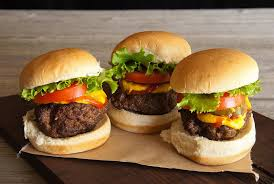
\includegraphics{resources/sliders_image.jpg}
\caption{}
\end{figure}

I was at a popular burger restaurant with two friends a while ago. On
the menu, there was an option to play ``Burger Roulette'' when you
ordered sliders. How it works is that if you order a plate of sliders (3
burgers on a plate), one of them will be loaded with very hot chilies.
As a result, the three of us each ordered a different plate of sliders
where one burger on each plate was loaded with very hot chilies.

The plan was that we would swap burgers between ourselves randomly as we
wanted to taste from each others' selection. I thought to myself, what
are the chances that I get all three spicy burgers on my plate?

\subsection{Assumptions}\label{assumptions}

\begin{itemize}
\item
  I presumed that you have absolutely no idea as to which burger
  contains the chilies. We would be naively swapping burgers.
\item
  There is a strict order of swapping. Player 1 and 2 will exchange
  burgers, then 2 and 3. Finally, 3 and 1 will swap.
\end{itemize}

\subsection{Script Logic}\label{script-logic}

I used the \texttt{tidyverse} and \texttt{doParallel} packages in
conducting the simulation. I used \texttt{ggalt} for added visualisation
features on top of \texttt{ggplot2}. I start by setting up a parallel
cluster and creating the burger swapping index function.

\begin{Shaded}
\begin{Highlighting}[]
\NormalTok{swapping_positions <-}\StringTok{ }\ControlFlowTok{function}\NormalTok{(number,min,max)\{}
  \KeywordTok{runif}\NormalTok{(}\DataTypeTok{n =}\NormalTok{ number,min,max) }\OperatorTok\StringTok{ }\KeywordTok{round}\NormalTok{(}\DataTypeTok{digits =} \DecValTok{0}\NormalTok{)}
\NormalTok{\}}
\end{Highlighting}
\end{Shaded}

A uniform random variable is created with a lower and upper bound of min
and max. This number is then rounded to an integer. This will be the
burger index that player A will choose from player B.

The script will use the \texttt{swapping\_positions} function to
exchange boolean elements between players for a given number of games at
a round size (r). An element is \texttt{TRUE} when it is a spicy burger.
The round size refers to how many swapping rounds there will be per
game. If r = 3 , the process as described in the second assumption will
be performed 3 times per game.

The script used is available as \texttt{spicy\_roulette.R}.

\subsection{Results}\label{results}

The simulation was conducted for round sizes up to 20 with each round
size being played for a total of 1 to 1000 games. The results are
plotted

\includegraphics{Naive_Simulation_Results_files/figure-latex/unnamed-chunk-2-1.pdf}

What immediately stands out are the two outliers at round size 16 and
20. These round sizes were played for 1 and 2 games respectively. The
script seemed to have produced pretty consistent results (see the plot
below) except for these two points. I decided to simulate a round size
of 16 and 20 for 1 and 2 games respectively in order to figure out how
unusual those points really are. I simulated the aforementioned burger
roulette descriptions 20000 times each. I generated the simulated
distributions below.

\includegraphics{Naive_Simulation_Results_files/figure-latex/unnamed-chunk-3-1.pdf}

The chances of observing the outlying point at round size of 16 is
approximately 1.22\% and the other outlier chance is 2.375\%. Although
these are all small probabilities, observing these points through the
main simulation is not unusual enough to bring the simulating procedure
into question.

Regardless, those points are clearly extreme outliers. They were
excluded from the plot to produce the second graph below.

\includegraphics{Naive_Simulation_Results_files/figure-latex/unnamed-chunk-4-1.pdf}

The colour scale according to game size proves to be quite useful in
this plot. You can clearly see that there is much more variation in the
results under low game sizes in green (\textless{}250) compared to large
game sizes in red (\textgreater{}750). Under large game sizes, the
percentage chance of success hovers around the same band of between
0.8\% and 1.3\%. Whilst this plot illustrates how the variance reduces
with increased game sizes, it doesn't show the density of the results
well. This is why I decided to plot a box plot for each round size in
the graph below.

\includegraphics{Naive_Simulation_Results_files/figure-latex/unnamed-chunk-5-1.pdf}

It can be clearly seen that 50\% of results for all game sizes for a
given round number occur approximately in the small band of 0.8\% and
1.3\%.

I attribute the small success rate due to the fact that you are naively
swapping burgers. As a result, it is quite likely that you undo your
progress (if you made any) with each success round. Under my
Assumptions, I stated a strict swapping order between players. I believe
that if I were to make that random, the chances of success would be even
lower as it would add another stochastic element that the players aren't
mitigating by their naive swapping.

So what is the long run probability of you sitting down and winning the
burger roulette? I ordered the results in ascending order and
constructed a 95\% confidence interval for the percentage chance of a
player winning the burger roulette.

\begin{Shaded}
\begin{Highlighting}[]
\NormalTok{ordered_results <-}\StringTok{ }\KeywordTok{sort}\NormalTok{(simulation_results}\OperatorTok{$}\NormalTok{all_spicy_chance)}
\NormalTok{lower_bound <-}\StringTok{ }\NormalTok{ordered_results[}\KeywordTok{length}\NormalTok{(ordered_results)}\OperatorTok{*}\FloatTok{0.025}\NormalTok{]}
\NormalTok{upper_bound <-}\StringTok{ }\NormalTok{ordered_results[}\KeywordTok{length}\NormalTok{(ordered_results)}\OperatorTok{*}\FloatTok{0.975}\NormalTok{]}
\end{Highlighting}
\end{Shaded}

\begin{verbatim}
## The 95% confidence interval for the true success rate is:[ 0 ; 2.671756 ]
\end{verbatim}

\subsection{Conclusion}\label{conclusion}

What we can say is that if you want to have exciting games with players
``winning'' the roulette, the round size is not that important , but you
need to have very low game sizes (\textless{}20). This maximises the
chances of getting a few games where a player has all three spicy
burgers. If spicy chilies are your kryptonite, you need not fear - you
are very likely not going to end up with all three spicy burgers.

\subsection{What I learnt}\label{what-i-learnt}

\begin{itemize}
\tightlist
\item
  Running simulations in parallel yields HUGE performance boosts. One
  just has to think through whether or not the problem is well suited to
  parallelisation.
\item
  Outliers should always be examined. I am glad that I looked at my two
  outlying points. It is important to figure out whether or not outliers
  are because of measurement errors , pure chance or a faulty algorithm.
\item
  I need to Git-good. This is the first mini-project that I used with
  Git. I use the Gitkraken client and it optimised my workflow nicely.
\end{itemize}


\end{document}
